\documentclass[12pt,halfline,a4paper,]{ouparticle}

% Packages I think are necessary for basic Rmarkdown functionality
\usepackage{hyperref}
\usepackage{graphicx}
\usepackage{listings}
\usepackage{color}
\usepackage{fancyvrb}
\usepackage{framed}

%% To allow better options for figure placement
%\usepackage{float}

% Packages that are supposedly required by OUP sty file
\usepackage{amssymb, amsmath, geometry, amsfonts, verbatim, endnotes, setspace}

% For code highlighting I think
\DefineVerbatimEnvironment{Highlighting}{Verbatim}{commandchars=\\\{\}}
\definecolor{shadecolor}{RGB}{248,248,248}
\newenvironment{Shaded}{\begin{snugshade}}{\end{snugshade}}
\newcommand{\AlertTok}[1]{\textcolor[rgb]{0.94,0.16,0.16}{#1}}
\newcommand{\AnnotationTok}[1]{\textcolor[rgb]{0.56,0.35,0.01}{\textbf{\textit{#1}}}}
\newcommand{\AttributeTok}[1]{\textcolor[rgb]{0.77,0.63,0.00}{#1}}
\newcommand{\BaseNTok}[1]{\textcolor[rgb]{0.00,0.00,0.81}{#1}}
\newcommand{\BuiltInTok}[1]{#1}
\newcommand{\CharTok}[1]{\textcolor[rgb]{0.31,0.60,0.02}{#1}}
\newcommand{\CommentTok}[1]{\textcolor[rgb]{0.56,0.35,0.01}{\textit{#1}}}
\newcommand{\CommentVarTok}[1]{\textcolor[rgb]{0.56,0.35,0.01}{\textbf{\textit{#1}}}}
\newcommand{\ConstantTok}[1]{\textcolor[rgb]{0.00,0.00,0.00}{#1}}
\newcommand{\ControlFlowTok}[1]{\textcolor[rgb]{0.13,0.29,0.53}{\textbf{#1}}}
\newcommand{\DataTypeTok}[1]{\textcolor[rgb]{0.13,0.29,0.53}{#1}}
\newcommand{\DecValTok}[1]{\textcolor[rgb]{0.00,0.00,0.81}{#1}}
\newcommand{\DocumentationTok}[1]{\textcolor[rgb]{0.56,0.35,0.01}{\textbf{\textit{#1}}}}
\newcommand{\ErrorTok}[1]{\textcolor[rgb]{0.64,0.00,0.00}{\textbf{#1}}}
\newcommand{\ExtensionTok}[1]{#1}
\newcommand{\FloatTok}[1]{\textcolor[rgb]{0.00,0.00,0.81}{#1}}
\newcommand{\FunctionTok}[1]{\textcolor[rgb]{0.00,0.00,0.00}{#1}}
\newcommand{\ImportTok}[1]{#1}
\newcommand{\InformationTok}[1]{\textcolor[rgb]{0.56,0.35,0.01}{\textbf{\textit{#1}}}}
\newcommand{\KeywordTok}[1]{\textcolor[rgb]{0.13,0.29,0.53}{\textbf{#1}}}
\newcommand{\NormalTok}[1]{#1}
\newcommand{\OperatorTok}[1]{\textcolor[rgb]{0.81,0.36,0.00}{\textbf{#1}}}
\newcommand{\OtherTok}[1]{\textcolor[rgb]{0.56,0.35,0.01}{#1}}
\newcommand{\PreprocessorTok}[1]{\textcolor[rgb]{0.56,0.35,0.01}{\textit{#1}}}
\newcommand{\RegionMarkerTok}[1]{#1}
\newcommand{\SpecialCharTok}[1]{\textcolor[rgb]{0.00,0.00,0.00}{#1}}
\newcommand{\SpecialStringTok}[1]{\textcolor[rgb]{0.31,0.60,0.02}{#1}}
\newcommand{\StringTok}[1]{\textcolor[rgb]{0.31,0.60,0.02}{#1}}
\newcommand{\VariableTok}[1]{\textcolor[rgb]{0.00,0.00,0.00}{#1}}
\newcommand{\VerbatimStringTok}[1]{\textcolor[rgb]{0.31,0.60,0.02}{#1}}
\newcommand{\WarningTok}[1]{\textcolor[rgb]{0.56,0.35,0.01}{\textbf{\textit{#1}}}}

% For making Rmarkdown lists
\providecommand{\tightlist}{%
  \setlength{\itemsep}{0pt}\setlength{\parskip}{0pt}}


% Part for setting citation format package: natbib
\usepackage{natbib}
\bibliographystyle{apsr}

% Part for setting citation format package: biblatex

% Pandoc header

\begin{document}

\title{Problem Set 3 Answer Key}

\author{%
\name{Joseph T. Ornstein}\address{University of Georgia}\email{\href{mailto:jornstein@uga.edu}{jornstein@uga.edu}}
}

\abstract{In this short paper, I demonstrate how to embed basic data analysis and
visualization into an \texttt{RMarkdown} document, creating a
reproducible workflow.}

\date{\today}

\keywords{RMarkdown; reproducible research; World Values Survey}

\maketitle



\hypertarget{introduction}{%
\section{Introduction}\label{introduction}}

The World Values Survey (WVS) is an extensive survey of cultural values;
Wave 7 of the survey interviewed 69578 people in 48 countries. It has
been cited in papers like
\citet{inglehartModernizationCulturalChange2000} and
\citet{minkovHofstedeFifthDimension2012}.

\hypertarget{results}{%
\section{Results}\label{results}}

Fig. \ref{fig:fig1} plots the number of respondents in each country who
say they are willing to fight for their country in the event of another
war. Note that the largest outlier is Japan, where a substantial
majority say no.

\begin{figure}[p]
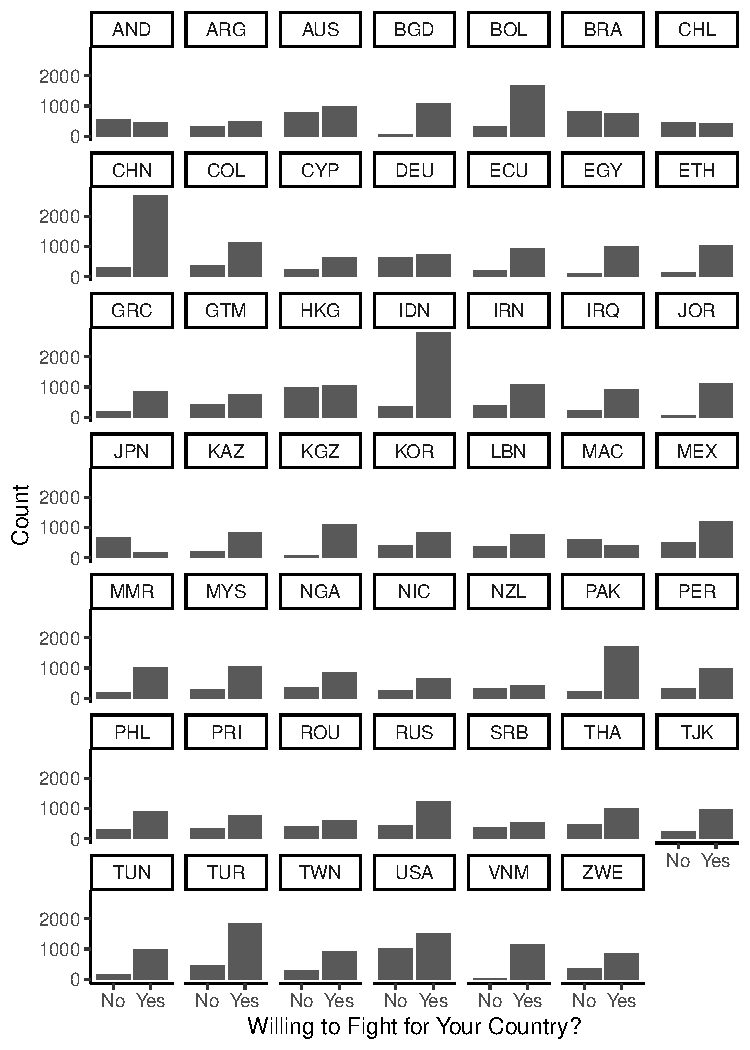
\includegraphics[width=1\linewidth]{problem-set-03-answer-key_files/figure-latex/fig1-1} \caption{Willingness to fight for one's country, by country}\label{fig:fig1}
\end{figure}




\renewcommand\refname{References}

\bibliography{refs.bib}



\end{document}
